%% -*- coding: utf-8 -*-
\documentclass[14pt,a4paper]{scrartcl} 
\usepackage[utf8]{inputenc}
\usepackage[english,russian]{babel}
\usepackage{indentfirst}
\usepackage{misccorr}
\usepackage{graphicx}
\usepackage{amsmath}
\usepackage{listings}

\begin{document}
\tableofcontents
\newpage
\section{Введение}
Для решения системы линейных алгебраических уравнений методом Гаусса была использована среда разработки Visual Studio 2022. Для оформления и написания отчёта использовался онлайн-компилятор LaTeX Overleaf


\newpage
\section{Алгоритм решения}
На первом этапе осуществляется так называемый прямой ход, когда путём элементарных преобразований над строками систему приводят к ступенчатой или треугольной форме, либо устанавливают, что система несовместна. А именно, среди элементов первого столбца матрицы выбирают ненулевой, перемещают его на крайнее верхнее положение перестановкой строк и вычитают получившуюся после перестановки первую строку из остальных строк, домножив её на величину, равную отношению первого элемента каждой из этих строк к первому элементу первой строки, обнуляя тем самым столбец под ним. После того, как указанные преобразования были совершены, первую строку и первый столбец мысленно вычёркивают и продолжают пока не останется матрица нулевого размера. Если на какой-то из итераций среди элементов первого столбца не нашёлся ненулевой, то переходят к следующему столбцу и проделывают аналогичную операцию.

На втором этапе осуществляется так называемый обратный ход, суть которого заключается в том, чтобы выразить все получившиеся базисные переменные через небазисные и построить фундаментальную систему решений, либо, если все переменные являются базисными, то выразить в численном виде единственное решение системы линейных уравнений. Эта процедура начинается с последнего уравнения, из которого выражают соответствующую базисную переменную (а она там всего одна) и подставляют в предыдущие уравнения, и так далее, поднимаясь по «ступенькам» наверх. Каждой строчке соответствует ровно одна базисная переменная, поэтому на каждом шаге, кроме последнего (самого верхнего), ситуация в точности повторяет случай последней строки.

В простейшем случае алгоритм выглядит так:
\begin{figure}[h!]
    \centering
    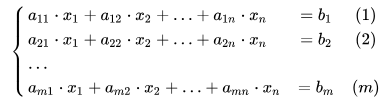
\includegraphics [width=0.6\textwidth]{formula1}\\
    
    \label{fig:pic2}
\end{figure}

Прямой ход:

\begin{figure}[h!]
    \centering
    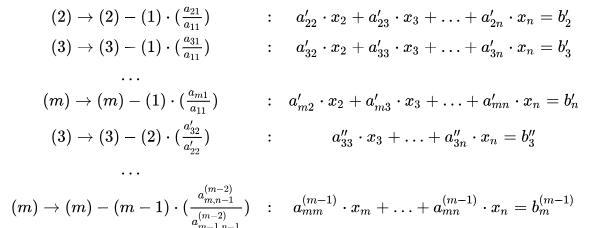
\includegraphics [width=0.6\textwidth]{formula2}\\
    
    \label{fig:pic2}
\end{figure}

\newpage


\section{Программа}
\lstinputlisting[language=C++, basicstyle=\footnotesize, inputencoding=cp1251, extendedchars=true]{Gauss.cpp}

Пользователь вводит количество уравнений и коэффициенты каждого уравнения, после чего программа решает систему методом Гаусса. В случае, если главный элемент матрицы равен нулю, программа меняет строки местами, чтобы избежать деления на ноль. После этого происходит нормализация главной строки и вычитание кратных ей строк из всех остальных для получения ступенчатой матрицы.

В конце программы выводится решение системы уравнений.

Использование векторов позволяет легко изменить размер матрицы и удобно хранить коэффициенты.
\begin{figure}[h!]
    \centering
    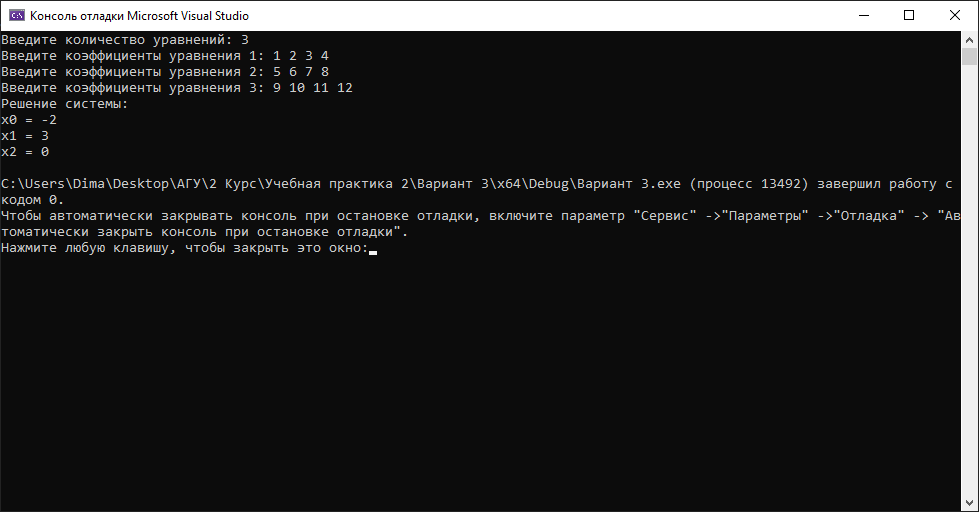
\includegraphics [width=0.9\textwidth]{Result}\\
    \caption{Результат выполнения программы}
    \label{fig:picResult}
\end{figure}

\newpage \section{Список используемой литературы}

\begin{enumerate}

    \item "Язык программирования C++. Базовый курс" Бьерн Страуструп - Издательство: «Питер», 2006, 1104с.
    \item "C++ Primer" Stanley Lippman, Josée Lajoie, Barbara E. Moo - 5-е издание, Издательство: «Альфа-книга», 2013 год, 976 страниц.
\end{enumerate}

\end{document}
